\section{Improving the Multiplexer and Mixed Signal Support}
\label{sec:improving}

TT05 split the mux into two parts to improve performance.
As each spine segment is now half as long, it will have half the capacitance.
We expect to reduce the round trip latency to around \qty{10}{\ns}.

For TT06, the Caravel harness will be replaced by OpenFrame~\cite{openframe}, an alternative harness provided by Efabless that uses the same padring but removes the RISC-V coprocessor.
This adds an extra \qty{5}{\mm\squared} more space for user designs, and an extra 12 pins that will be used for analog.

For increased safety, all designs will be power-gated, which will allow designers to take more risks or use custom flows.

Analog and mixed-signal designs will be enabled by adding an analog multiplexer based on transmission gates~\cite{transmissiongates}. 
This allows up to 192 designs to share the 8 analog pins between them.
The transmission gates were tested as part of an experimental analog submission to TT05 shown in Fig.~\ref{fig:transmission_gate_TT05}.

\begin{figure}[!t]
\centering
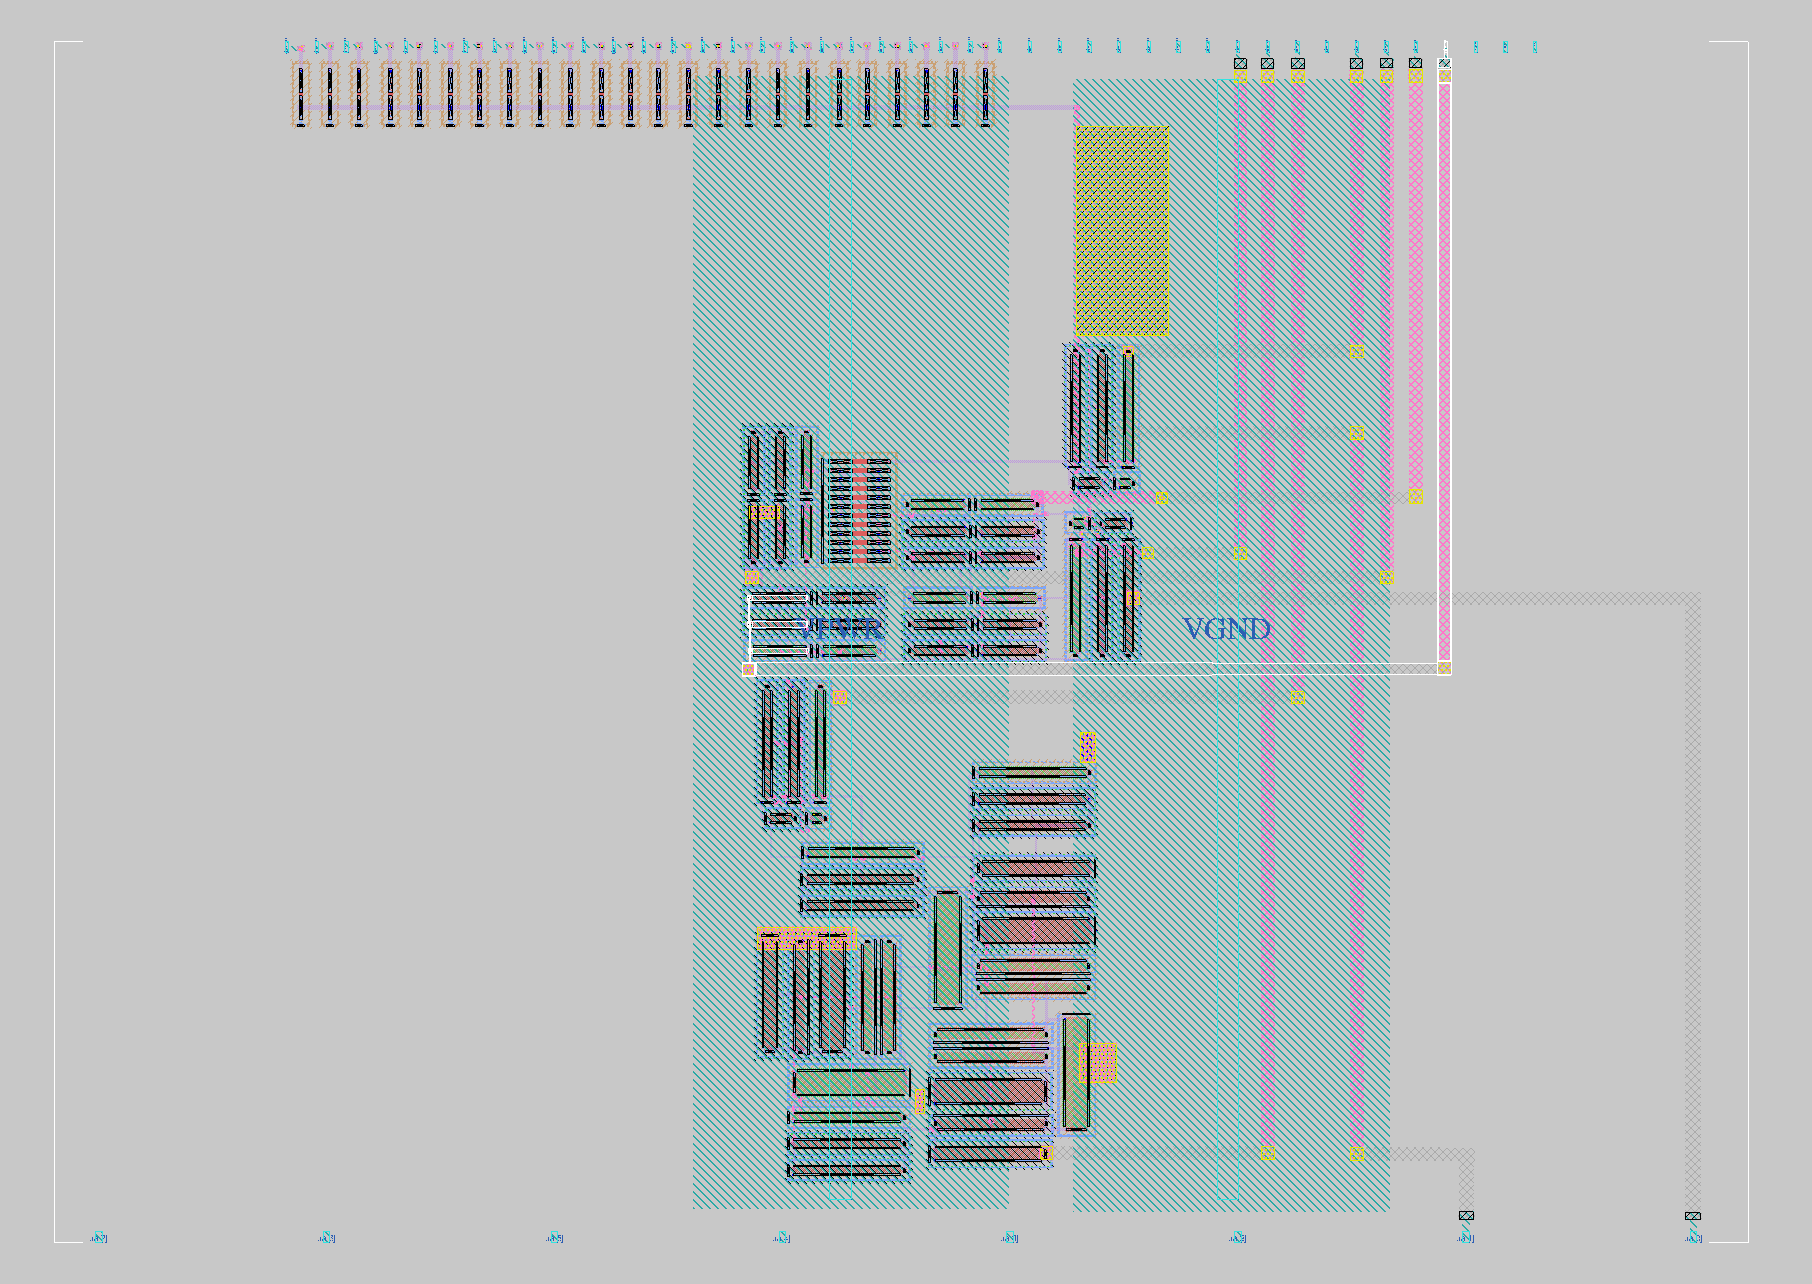
\includegraphics[width=\columnwidth]{./Figs/tt05_transmission_gate.png}
\caption{Analog design submitted to TT05 with a transmission gate high-lighted (auto-placed and auto-routed using an experimental analog P\&R tool).}
\label{fig:transmission_gate_TT05}
\end{figure}

TT06 is planned to open for digital designs at the end of January 2024, for analog designs at the end of February, and to close on April 19th, 2024.
